\documentclass[10pt,a4paper]{article}

\usepackage{fullpage}
\usepackage{setspace}
\usepackage{parskip}
\usepackage{titlesec}
\usepackage[section]{placeins}
\usepackage{xcolor}
\usepackage{breakcites}
\usepackage{lineno}
\usepackage{hyphenat}





\PassOptionsToPackage{hyphens}{url}
\usepackage[colorlinks = true,
            linkcolor = blue,
            urlcolor  = blue,
            citecolor = blue,
            anchorcolor = blue]{hyperref}
\usepackage{etoolbox}
\makeatletter
\patchcmd\@combinedblfloats{\box\@outputbox}{\unvbox\@outputbox}{}{%
  \errmessage{\noexpand\@combinedblfloats could not be patched}%
}%
\makeatother


\usepackage{natbib}




\renewenvironment{abstract}
  {{\bfseries\noindent{\abstractname}\par\nobreak}\footnotesize}
  {\bigskip}

\titlespacing{\section}{0pt}{*3}{*1}
\titlespacing{\subsection}{0pt}{*2}{*0.5}
\titlespacing{\subsubsection}{0pt}{*1.5}{0pt}


\usepackage{authblk}


\usepackage{graphicx}
\usepackage[space]{grffile}
\usepackage{latexsym}
\usepackage{textcomp}
\usepackage{longtable}
\usepackage{tabulary}
\usepackage{booktabs,array,multirow}
\usepackage{amsfonts,amsmath,amssymb}
\providecommand\citet{\cite}
\providecommand\citep{\cite}
\providecommand\citealt{\cite}
% You can conditionalize code for latexml or normal latex using this.
\newif\iflatexml\latexmlfalse
\providecommand{\tightlist}{\setlength{\itemsep}{0pt}\setlength{\parskip}{0pt}}%

\AtBeginDocument{\DeclareGraphicsExtensions{.pdf,.PDF,.eps,.EPS,.png,.PNG,.tif,.TIF,.jpg,.JPG,.jpeg,.JPEG}}

\usepackage[utf8]{inputenc}
\usepackage[english,ngerman,italian]{babel}



\usepackage{float}






% Edit this header.tex file to include frontmatter definitions and global macros

% Add here any LaTeX packages you would like to load in all document blocks
% \usepackage{xspace}

% Add here any LaTeX macros you would like to load in all document blocks
% \def\example{This is an example macro.}

% -----

\iflatexml
% Add here any LaTeXML-specific commands

% -----

\else
% Add here any export style-specific LaTeX commands. These will only be loaded upon document export. 
% \paperfield{Subject domain of my document}
% \keywords{keyword1, keyword2}
% \corraddress{Author One PhD, Department, Institution, City, State or Province, Postal Code, Country}
% \fundinginfo{Funder One, Funder One Department, Grant/Award Number: 123456.}
\fi


\begin{document}

\title{Energia cinetica di rotazione}



\author[1]{Dennis Angemi}%
\author[1]{Giuseppe Di Silvestre}%
\author[1]{Federica Ingrassia}%
\author[1]{Giulia De Luca}%
\affil[1]{Dipartimento di Fisica e Astronomia "Ettore Majorana" - Università degli Studi di Catania}%


\vspace{-1em}



  \date{}


\begingroup
\let\center\flushleft
\let\endcenter\endflushleft
\maketitle
\endgroup





\selectlanguage{italian}
\begin{abstract}
Si \selectlanguage{ngerman}è determinato il valore del momento di inerzia di una ruota metallica
dalla misura dei tempi impiegati da un carrello a percorrere un tratto
di un piano inclinato (sfruttando il principio di conservazione
dell'energia). Il valore così ottenuto risulta essere in buon accordo
col dato normalmente accettato.%
\end{abstract}\selectlanguage{ngerman}%



\sloppy


\section*{\texorpdfstring{{Introduzione e cenni
teorici}}{Introduzione e cenni teorici}}

{\label{876971}}

Si consideri un carrello di massa~\(m_c\)~ avente 4 ruote di
raggio~\(r\) alle quali vengono aggiunte 2 ruote posteriori
di raggio~\(R\) e massa~\(M\) vincolate in
modo tale da non entrare in contatto con la superficie del piano
inclinato.

Trascurando le forze di attrito, sul sistema agiscono le forze
illustrate in~{\ref{240030}}\selectlanguage{italian}
\begin{figure}[H]
\begin{center}
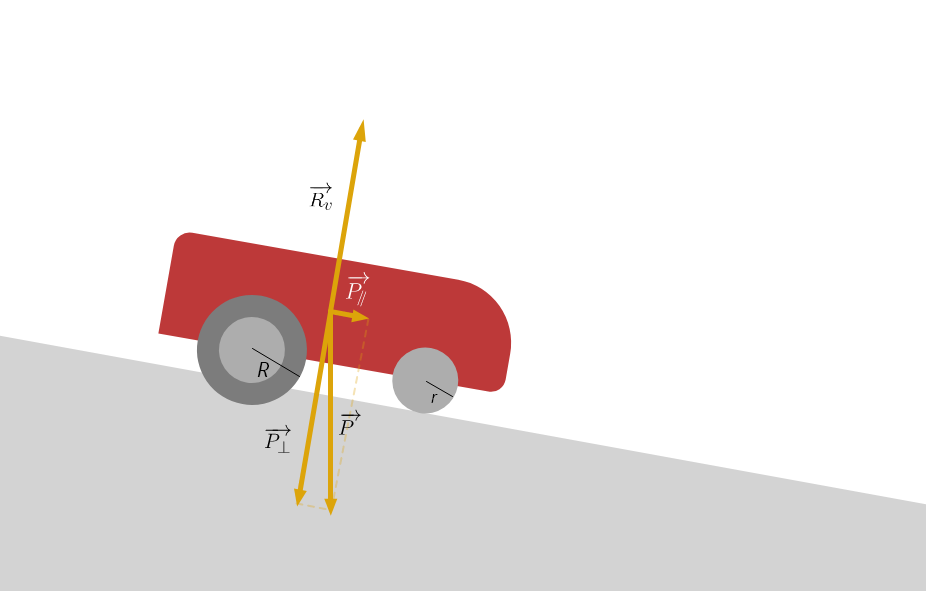
\includegraphics[width=0.70\columnwidth]{figures/diagramma/diagramma}
\caption{{Diagramma delle forze
{\label{240030}}%
}}
\end{center}
\end{figure}

Il carrello si muove quindi di moto rettilineo uniformemente accelerato
per effetto della componente della forza peso ~\(\overrightarrow{P_{\parallel}}\)
parallela al piano. Fissati~\(s_0=0\) e~\(t_0=0\),
valgono le seguenti equazioni del moto

\begin{equation} \begin{cases}v_{1}=a_1 t_{1}\\ s=\frac{1}{2}a_{1} t_{1}^{2}\\ \end{cases}\ \\  \end{equation}

\begin{equation} \begin{cases}v_{2}=a_2 t_{2}\\ s=\frac{1}{2}a_{2} t_{2}^{2}\\ \end{cases}\ \\  \end{equation}

dalle quali si ottiene~\(v_1=\frac{2s}{t_1}\)~,~\(v_2=\frac{2s}{t_2}\).

Per il principio di conservazione dell'energia:

\begin{equation}
    \begin{cases}
      m_{tot} g h = \frac{1}{2} m_{tot} v_1^2\\
      m_{tot} g h = \frac{1}{2} m_{tot} v_2^2 + \frac{1}{2}(2 I \omega^2 )\\
    \end{cases}\
\end{equation}

in cui:

\begin{itemize}
\tightlist
\item
  \(v_1\)~rappresenta la velocit\selectlanguage{ngerman}à finale del carrello al
  quale sono vincolate posteriormente due ruote aggiuntive di
  massa~\(M\)e raggio~\(R\) \emph{libere} in
  modo tale che \emph{non} ruotino;
\item
  \(v_2\)~rappresenta la velocità finale del carrello al
  quale sono oppurtunamente vincolate le ruote (precedentemente
  descritte)~\emph{bloccate~}in modo tale che \emph{ruotino}
  solidalmente~alle ruote di raggio~\(r\);
\item
  \(\omega=\frac{v_2}{r}\) è la velocità angolare delle ruote di
  raggio~\(r\).
\end{itemize}

La prima equazione del sistema (3) esprime il principio di conservazione
dell'energia meccanica nella configurazione in cui l'energia potenziale
iniziale corrisponde all'energia cinetica finale in quanto i momenti di
inerzia delle ruote di raggio~\(r\) influiscono minimamente
sul sistema e viene trascurato l'attrito tra le ruote e le rotaie.~

Nella seconda equazione del sistema (3), oltre al termine che esprime
l'energia cinetica traslazionale, compare il termine dell'energia
cinetica rotazionale che verrà sfruttato nella determinazione del
momento di inerzia~\(I\)delle ruote di
raggio~\(R\). Infatti, risolvendo il sistema di equazioni
(3) si ottiene

\[I=\frac{1}{2}m_{tot} r^2\left[\left(\frac{t_2}{t_1}\right)^2-1\right].\]

Il momento di inerzia nel caso di un punto materiale è definito come il
prodotto della massa per il quadrato della distanza del punto dell'asse
di rotazione. Il momento di inerzia I~di un corpo dipende dalla
geometria di quest'ultimo per tanto approssimiamo la geometria di una
ruota ad un parallelipedo solido di massa \emph{m} e raggio \emph{R}.
Noi otterremo tale valore sfruttando il principio di conservazione
dell'energia e lo confronteremo con il valore ottenuto considerando le
caratteristiche geometriche della ruota (cilindro).

\section*{Apparato sperimentale e procedura di
misura}

{\label{507351}}

\subsection*{Descrizione}

{\label{588451}}

L'apparato sperimentale è costituito da una rotaia inclinata sulla quale
si muove un carrello (precedentemente descritto) e da due fotocellule
azionate nell'istante del passaggio del carrello in modo tale da
determinare l'intervallo di tempo impiegato dal corpo a percorrere la
distanza \(s=s_2 - s_1\).

Sono state effettuate 40 osservazioni (Table 1):

\begin{itemize}
\tightlist
\item
  20 misurazioni dell'intervallo di tempo nella configurazione ``ruote
  libere'';
\item
  20 misurazioni dell'intervallo di tempo nella configurazione ``ruote
  bloccate''.
\end{itemize}

\par\null\selectlanguage{italian}
\begin{figure}[H]
\begin{center}
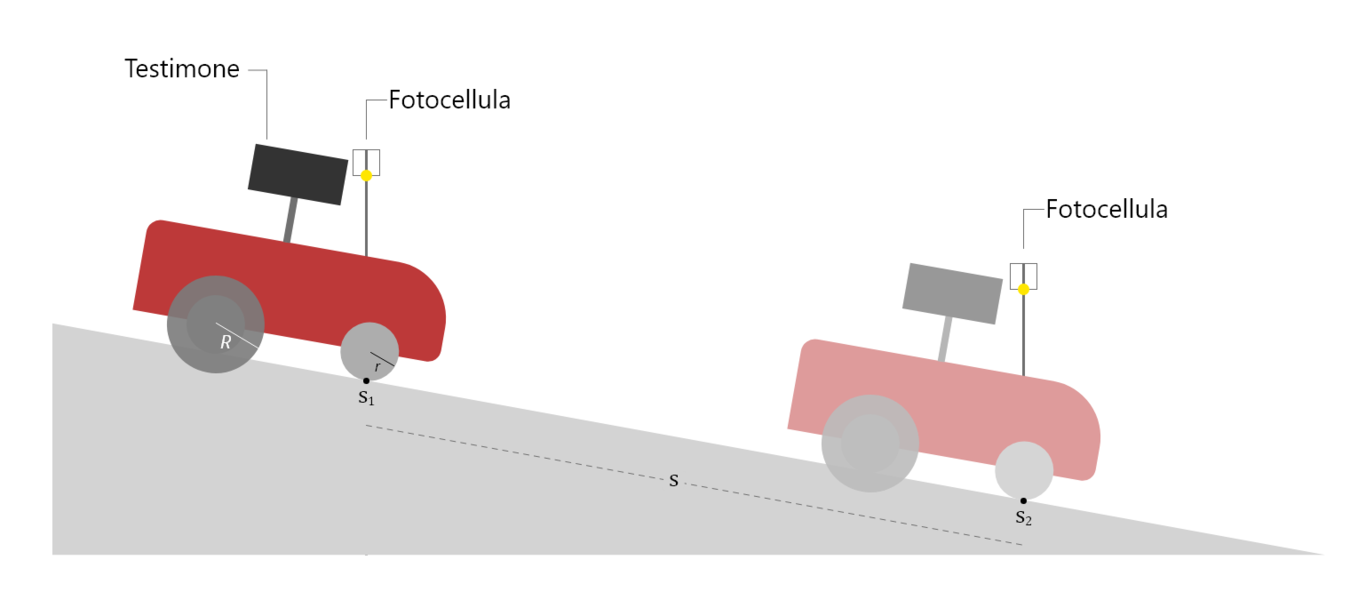
\includegraphics[width=0.91\columnwidth]{figures/img/apparato-sperimentale}
\caption{{Apparato sperimentale
{\label{577816}}%
}}
\end{center}
\end{figure}

\subsection*{Strumenti di misura}

{\label{970197}}

Le misurazioni riportate nei prossimi paragrafi sono state effettuate
adoperando gli strumenti le cui caratteristiche sono di seguito
riassunte:\selectlanguage{italian}
\begin{longtable}[]{@{}lll@{}}
\toprule
Strumento & Sensibilit\selectlanguage{ngerman}à & udm\tabularnewline
\midrule
\endhead
Bilancia & 0.0001 & kg\tabularnewline
Flessometro & 0.001 & m\tabularnewline
Calibro cinquantesimale & 0.00005 & m\tabularnewline
Calibro ventesimale & 0.00002 & m\tabularnewline
Cronometro & 0.001 & s\tabularnewline
\bottomrule
\end{longtable}

\section*{Analisi dei dati ed analisi degli
errori}

{\label{151909}}

Al fine di determinare~~\(I\) mediante l'eq. (4), si
calcola il tempo medio impiegato dal carrello a percorrere la
distanza~\(s\)

\(\langle t_1 \rangle = \sum_{i=1}^{20} t_{1i}\)

\(\langle t_2 \rangle = \sum_{i=1}^{20} t_{2i}\)

Sostituendo nella (4) si ottiene\[I=\frac{1}{2}m_{tot} r^2\left[\left(\frac{\langle{t_2}\rangle}{\langle{t_1}\rangle}\right)^2-1\right].\]

Propagazione degli errori

\[\delta I = \left | \frac{\partial I}{\partial r} \right |\delta r + 3 \left | \frac{\partial I}{\partial m} \right | \delta m + \left | \frac{\partial I}{\partial t_2} \right | \delta t + \left | \frac{\partial I}{\partial t_1} \right |\delta t\]

\[\delta I = \left [ \left ( \frac{\langle t_2 \rangle}{\langle t_1 \rangle} \right) ^2 -1 \right] \left (m_{tot} r \delta r + \frac{3}{2} r^2 \delta m \right) + r^2 m_{tot} \left ( \frac{\langle t_2 \rangle}{\langle t_1 \rangle} \right) ^2 \left ( \frac{1}{\langle t_1 \rangle} +  \frac{1}{\langle t_2 \rangle} \right) \delta t\]

Confrontiamo il valore ottenuto con~

\[I'=\frac{m_1R^2}{2}\]

Si procede a studiare l'incertezza di quest'ultimo valore

\[\delta I' = \frac{\partial I'}{\partial m_1} \delta m_1 + \frac{\partial I'}{\partial R} \delta R=R \left ( \frac{R \delta m}{2} + m_1 \delta R \right )\]

\section*{Risultati}

{\label{420816}}

Scrivere decentemente questo paragrafo

Dalla (4) si ottiene~~\(I=(1.37 \pm 0.01) \times 10^{-3}\,kg\,m^2\)

Dalla (7) si ottiene~\(I'=(1.3689 \pm 0.0001) \times 10^{-3} \,kg\,m^2\)

\(I'\) risulta essere pi\selectlanguage{ngerman}ù preciso dato il maggior numero di
cifre significative; i valori di~\(I\)
e~\(I'\) risultano essere in buon accordo

\section*{Appendice A}

{\label{501222}}

\textbf{Tabella
1~}(\href{https://raw.githubusercontent.com/dennisangemi/lab1-dfa/main/exp-1/experimental-data-1.csv}{Download
CSV})\selectlanguage{italian}
\begin{longtable}[]{@{}lllll@{}}
\toprule
index & t1 & t2 & incertezza & udm\tabularnewline
\midrule
\endhead
1 & 1.545 & 2.029 & 0.001 & s\tabularnewline
2 & 1.545 & 2.042 & 0.001 & s\tabularnewline
3 & 1.546 & 2.032 & 0.001 & s\tabularnewline
4 & 1.545 & 2.022 & 0.001 & s\tabularnewline
5 & 1.541 & 2.027 & 0.001 & s\tabularnewline
6 & 1.545 & 2.027 & 0.001 & s\tabularnewline
7 & 1.536 & 2.004 & 0.001 & s\tabularnewline
8 & 1.542 & 2.028 & 0.001 & s\tabularnewline
9 & 1.536 & 2.035 & 0.001 & s\tabularnewline
10 & 1.542 & 2.025 & 0.001 & s\tabularnewline
11 & 1.533 & 2.026 & 0.001 & s\tabularnewline
12 & 1.531 & 2.021 & 0.001 & s\tabularnewline
13 & 1.539 & 2.023 & 0.001 & s\tabularnewline
14 & 1.536 & 2.014 & 0.001 & s\tabularnewline
16 & 1.539 & 2.021 & 0.001 & s\tabularnewline
15 & 1.541 & 2.034 & 0.001 & s\tabularnewline
17 & 1.541 & 2.015 & 0.001 & s\tabularnewline
18 & 1.547 & 2.018 & 0.001 & s\tabularnewline
19 & 1.534 & 2.015 & 0.001 & s\tabularnewline
20 & 1.537 & 1.996 & 0.001 & s\tabularnewline
\bottomrule
\end{longtable}

\textbf{Tabella
2~}(\href{https://raw.githubusercontent.com/dennisangemi/lab1-dfa/main/exp-1/experimental-data-2.csv}{Download
CSV})\selectlanguage{italian}
\begin{longtable}[]{@{}lllll@{}}
\toprule
descrizione & valore & incertezza & udm & strumento\tabularnewline
\midrule
\endhead
Massa ruota dx di raggio R & 1.1205 & 0.0001 & kg &
Bilancia\tabularnewline
Massa ruota sx di raggio R & 1.1234 & 0.0001 & kg &
Bilancia\tabularnewline
Massa carrello (privo di ruote di raggio R) & 3.8871 & 0.0001 & kg &
Bilancia\tabularnewline
Diametro ruote di raggio r & 0.04965 & 0.00005 & m & Calibro
cinquantesimale\tabularnewline
Diametro ruote di raggio R & 0.09886 & 0.00002 & m & Calibro
ventesimale\tabularnewline
\bottomrule
\end{longtable}

\section*{Note}

{\label{277394}}

\subsection*{Software utilizzati}

{\label{321913}}

\begin{itemize}
\tightlist
\item
  \textbf{MATLAB}: Data Analysis
\item
  \textbf{Google Spreadsheet}: Data entry
\item
  \textbf{Adobe Experience Design}: Images designing
\item
  \textbf{GitHub}: Resource sharing
\end{itemize}

\subsection*{Risorse condivise}

{\label{314313}}

\begin{itemize}
\tightlist
\item
  \href{https://github.com/dennisangemi/lab1-dfa/tree/main/exp-1}{GitHub
  Repository}
\item
  \href{https://drive.matlab.com/sharing/2e64529c-09bc-4c03-8059-75fa50e48ce6/exp_01.mlx}{MATLAB
  livescript}
\end{itemize}

\section*{Bibliografia}

{\label{333834}}

\begin{itemize}
\tightlist
\item
  Taylor,~ J. (1999).~\emph{Introduzione all'analisi degli errori: Lo
  studio delle incertezze nelle misure fisiche.~}Zanichelli
\item
  Bevington P. (2002).~\emph{Data Reduction and Error Analysis for the
  Physical Sciences.~} McGraw-Hill Education ~
\end{itemize}

\par\null

\selectlanguage{italian}
\FloatBarrier
\end{document}

